%% print or electronic
\documentclass[ms,electronic,double]{nuthesis}

%% Needed to typset the math in this sample
\usepackage{amsmath}
\usepackage{amsfonts}
%% Let's use a different font
\usepackage[sc,osf]{mathpazo}

%% Makes things look better
\usepackage{microtype}

%% Makes things look better
\usepackage{booktabs}

%% Gives us extra list environments
\usepackage{paralist}

%% Be able to include graphicsx
\usepackage{graphicx}
%% Needed to display code 
\usepackage{listings}
\usepackage{algorithmic}
\usepackage{algorithm}
\usepackage{subfig}
\usepackage{url}
\usepackage{placeins}

%% I like darker colors
\usepackage{color}
\definecolor{dark-red}{rgb}{0.6,0,0}
\definecolor{dark-green}{rgb}{0,0.6,0}
\definecolor{dark-blue}{rgb}{0,0,0.6}
\definecolor{dark-purple}{rgb}{0.5,0,0.35} 
\definecolor{light-grey}{rgb}{0.9,0.9,0.9}

%% If you use hyperref, you need to load memhfixc *after* it.
%% See the memoir docs for details.
\usepackage[%
pdfauthor={Kartik Vedalaveni},
pdftitle={Adaptive Co-Scheduler for highly Dynamic Resource},
pdfsubject={Thesis},
pdfkeywords={LaTeX, Thesis, University of Nebraska, Intelligent Co-Scheduler},
linkcolor=dark-blue,
pagecolor=dark-green,
citecolor=dark-blue,
urlcolor=dark-red,
colorlinks=true,
backref,
plainpages=false,% This helps to fix the issue with hyperref with page numbering
pdfpagelabels% This helps to fix the issue with hyperref with page numbering
]{hyperref}

%Listings color code
\lstset{
language=c,
basicstyle=\ttfamily,
keywordstyle=\color{dark-purple}\bfseries,
stringstyle=\color{dark-red},
commentstyle=\color{dark-green},
morecomment=[s][\color{dark-blue}]{/**}{*/},
numbers=left,%left, right, none
numberstyle=\tiny\color{black},
stepnumber=1,
numbersep=10pt,
tabsize=4,
showspaces=false,
showstringspaces=false,
frame=none,
backgroundcolor=\color{light-grey}
}

%% Needed by memoir to fix things with hyperref
\usepackage{memhfixc}


\begin{document}
\frontmatter
\title{Adaptive Co-Scheduler for highly Dynamic Resource}
\author{Kartik Vedalaveni}
\adviser{Dr. David Swanson}
\adviserAbstract{Dr. David Swanson}
\major{Computer Science}
\degreemonth{May}
\degreeyear{2013}
\college{Graduate College}
\university{University Of Nebraska}
\city{Lincoln}
\state{Nebraska}
\doctype{Thesis}
\degree{Master Of Science}
\degreeabbreviation{M.S}
\maketitle

\begin{abstract}
Schedulers come with a plethora of features and 
options for customization that fulfill myriad goals of  
clusters and data centers . Most state of the art schedulers do not take into account load of resources 
like RAM, I/O or Network for scheduling purposes. Often there is a need to extend these schedulers to solve 
situations arising from these new use cases either by writing a plugin or by Co-Scheduling. One such 
issue is when any resource like I/O, RAM or Network is
overwhelmed and performance degradation that occurs as a result of it . With an increase in the number 
of entities concurrently using the resource, there is a 
need to monitor and schedule concurrent and unmanaged access to any given resource to prevent 
degradation.These issues that we encounter in real life at Holland Computing Center (CITE) are the 
basis and motivation for tackling this problem and develop an adaptive approach for scheduling 
that is aware of multi-resource throttling, load-balancing across multiple sites and degradation 
with a goal to run clusters at high efficiency and share resources fluidly. 
\end{abstract}

\begin{dedication}
Dedicated to 
\end{dedication}

\begin{acknowledgments}
Thanks
\end{acknowledgments}

\tableofcontents
\newpage
\listoffigures
\listoftables


%%   mainmatter is needed after the ToC, (LoF, and LoT) to set the
%%   page numbering correctly for the main body
\mainmatter

\chapter{Introduction}
Grid Computing as defined by wikipedia is the federation of computer resources from multiple locations
to reach a common goal. The resources come in the form of hardware 
and software that allows us to submit jobs, run the jobs and monitor the jobs on the grid. 
Universities usually have multiple clusters across their campus and these are 
owned by different departments but stand united under the banner of the university.
Campus grids can be thought of as mini grids in which jobs are spanned across multiple clusters
 based on the need of the user and available computing infrastructure 
across multiple clusters within the computing resources across the university.

Modern schedulers used in clusters provide numerable features for policy making, resource management 
and scheduling, the problem of cluster 
performance degradation that occurs when either of the resource is throttled is a problem that hasn't been 
addressed. The problem of performance degradation when many jobs are scheduled on a single system 
are either based on processor equivalence or based on the number of processor slots. Some of 
these schedulers like maui (CITE) are smart enough to take into account contention of other 
resources like RAM but ultimately convert the 2D vector values of CPU and RAM 
into single scalar value which drop to hard-coding the value or presenting these resources
in a ratio which makes us question effectiveness of such scheduling mechanism. 

At Holland Computing Center present in University Of Nebraska-Lincoln, we're 
tackling this issue of cluster degradation caused by 
over exploitation of one or more resource and we've come up with a solution by adaptively scheduling 
such highly dynamic resource on the grid across multiple sites by adaptively scaling with respect to
degradation that is encountered and scheduling based on least turnaround time of the sites which would help increase 
the throughput of the overall Co-Scheduler which also loadbalances.

Existing schedulers depend on the availability of resources and frequent polling 
of it to determine the slots of scheduling. It should be noted that state of the art 
schedulers like maui/torque, slurm, condor take into account only CPU as a 
resource and the resources like RAM, I/O or Network are either ignored or 
their resource equivalent is converted into a scalar values which isn't an effective way of tackling the 
multiple resource scheduling problem as this might result in scheduling excessive jobs 
on single machine in case of schedulers ignoring the resource and loss of 
effective resources when schedulers convert the resource allocation into scalar 
values which means for example it'll be pre-assigned on every node that 1 CPU-CORE will have 2 GB of
memory this kind of pre-assignment seems like its addressing the resource degradation of RAM but suffers 
from the above mentioned problems.
We take a turnaround time approach to measure degradation, we define a resource 
to be degraded if and when we submit jobs that results in increasing the 
turnaround time by 25\% . It must be 
noted that there isn't explicit measurement of individual resources of RAM, I/O, 
Network and CPU, there are no resource managers keeping track of these resource allocations. 
The Co-Scheduler is driven by the fact that turnaround time increases when 
concurrent jobs accessing these resources reaches a threshold value which in-turn causes 
degradation and this is the basis for our scheduling.

\begin{figure}[htbp!]
\begin{center}
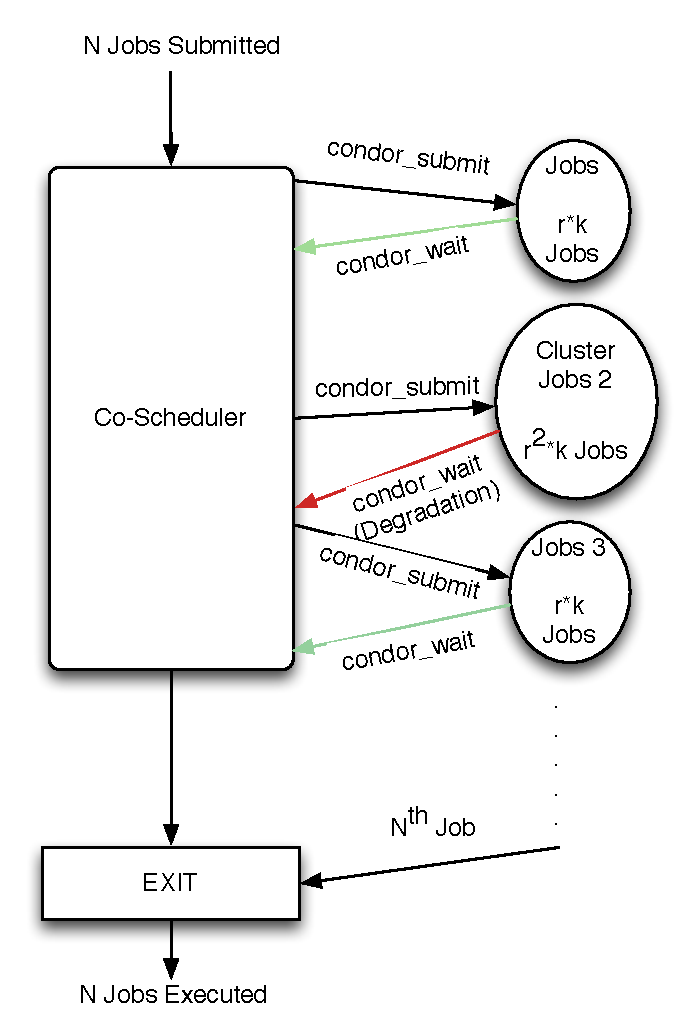
\includegraphics[scale=0.75]{images/degradation_detection}
\caption{Degradation occurrence: Co-Scheduling}
\label{fig:degradationdetect-intro}
\end{center}
\end{figure}

One aspect to Co-Scheduler is degradation detection and management by adapting 
to the throttling of a resource, another aspect is to efficiently distribute jobs 
across multiple sites which increases the throughput of the workload
. The Co-Scheduler adapts to degradation by backing off submission rates and waiting for random
period of time for the next incremental submission and efficiently 
distributes the jobs and load-balances across multiple sites, thus submitting more 
jobs to a site with lesser turnaround time and also ensuring to submit lesser 
jobs to the sites with larger turnaround time thus efficiently load-balancing 
across multiple sites on a grid and improving throughput.

In the figure \ref{fig:degradationdetect-intro}, if C1 is called job propagation factor and k is initial number of 
jobs submitted then we can see that on each iteration we're adding $k = C1 * k$ jobs and on the
next iteration if we have a degraded system then we submit $k=k/C1$ amount of 
jobs.

Finally, since the grid environment is a heterogeneous environment, it's absolutely necessary
to use API that are available on all the systems across the grid. To implement such a Co-Scheduler
 we limit ourselves to condor based clusters and utilize libcondorapi. The result is a threaded Co-Scheduler 
that submits to multiple sites concurrently and is aware of multiple-resource degradation and
loadbalances efficiently across multiple sites of the grid. 

Please note that all the references to the Co-Scheduler in this thesis refers to the adaptive Co-Scheduler designed 
by us.  
\section{Co-Scheduler}

DHTC environment


%% Thesis goes here
\chapter{Background}

\section{High-Throughput Computing} High Throughput Computing, HTC is defined as 
a computing environment that delivers large amounts of computational
power over a long period of time.  The important factor being over a long period of time which 
differentiates HTC from HPC which focuses on getting large amount of work done in small amount of time.
The workloads that run on condor system doesn't have an objective of  how fast the job can be completed 
but how many times can the job be run in the next few months.In another definition of HTC, European Grid  
Infrastructure defines HTC as a computing paradigm that focuses on the efficient 
execution of large number of loosely coupled tasks. (CITE)


\section{HTCondor} HTCondor is a distributed system developed by HTCondor team at the 
University of Wisconsin-Madison. It provides High-Throughput Computing environment to sites 
that foster research computing and enables sites to share computing resources when 
computers are idle at a given site. HTCondor system includes a batch queuing 
system,scheduling policy, priority scheme, and resource classifications for a pool of 
computers, which is mainly used for compute-intensive jobs. HTCondor runs on both
 UNIX and windows based workstations that are all connected by a network.  
Although there are other batch schedulers out there for dedicated machines. 
The power of condor comes from  the fact that  the amount of compute power 
represented by sum total of all the 
 non-dedicated desktop workstations sitting on people's desks is sometimes far 
 greater than the compute power of dedicated central resource. There are many 
 unique tools and capabilities in HTCondor which make utilizing resources from 
 non-dedicated systems effective. These capabilities include process checkpoint 
 and migration, remote system calls and ClassAds. HTCondor suit also includes a 
 powerful resource manager with an efficient match-making mechanism that is 
 implemented via ClassAds, which makes HTCondor lucid when compared with other 
 compute schedulers.
 
 
\section{Open Science Grid} Open Science Grid(OSG), provides service and support 
for resource providers and scientific institutions using a distributed fabric of 
high throughout computational services. OSG was created to facilitate data analysis from the 
Large Hadron Collider . OSG doesn't own resources but provides software and services to 
users and enables opportunistic usage and sharing of resources among resource providers.
The main goal of OSG is to advance science through open distributed computing. 
The OSG provides multi-disciplinary partnership to federate local, regional, community and 
national cyber-infrastructures to meet the needs of research and academic communities at all scales.

OSG provides resources and directions to Virtual Organizations(VO's) for the purposes of LHC experiments
and HTC in general. \\

Building a OSG site requires listing background and careful planning. The major 
components of a OSG site includes a Storage Element and Compute Element. \\

Storage elements (SE) manage physical systems, disk caches and hierarchical mass storage 
systems, its an interface for grid jobs to underlying storage Storage Resource Management protocol and Globus 
Grid FTP protocol and others, A storage element requires an underlying storage system like hadoop, xrootd
and a GridFTP server and an SRM interface.\\

A Compute Element(CE) allows grid users to run jobs on your site. It provides a 
bunch of services when run on the gatekeeper. The basic components include 
the GRAM and GridFTP on the same CE host to successfully enable file transfer 
mechanisms of Condor-G.\\

\section{Grid Computing}

\section{Globus}

We delegate our identification on the grid. \emph{voms-proxy-init}
is used to generate voms proxy at the submit host, we can specify \texttt{--voms} as our 
virtual organization, hcc:/hcc in this case and \texttt{--hours} as the number of hours the proxy would be 
active/valid, it must be ensured that the proxy period is approximately greater than the 
length of period of runtime of jobs for smooth running of jobs.

HTCondor-G is the grid environment, when jobs are sent across grid universe using 
Globus software. Globus toolkit provides support for building grid systems. 
Submitting, managing and executing jobs have same capabilities in both HTCondor 
and HTCondor-G world. Globus provides fault tolerant features to HTCondor-G 
jobs.GRAM is Grid Resource Allocation and Management protocol, supports remote 
submission of computational request.

gt2 is an initial GRAM protocol which is used in Globus Toolkit version 1 and 
2. gt2 is also referred to as the pre-web services GRAM or GRAM2.

gt5 is the latest GRAM protocol, which is an extension of GRAM2 and is intended 
to be more scalable and robust, referred to as GRAM5.


\section{Batch Scheduling}


\chapter{Related Work}

\section{Comparison of existing mechanisms}
There might be situations where we can have multiple condor pools and some of 
the pools might have many idle slots that are available for utilization. To efficiently utilize the resources across pools condor provides 
mechanisms like condor flocking and condor job router. These mechanisms 
provide similar functionality to the Co-Scheduler that I designed here. In the following sections, we compare 
and evaluate these mechanisms with the design and functionality of Co-Scheduler.

\subsection{Condor Flocking}
Flocking refers to a mechanism where jobs that cannot run in its own condor pool 
due to lack of resources runs in another condor pool where resources are 
available. Condor flocking enables load sharing between pools of computers. As 
pointed out by Campus Grids Thesis[CITE 3.1.2]  flocking helps balance large workflows across different pools but not 
necessarily the jobs across these pools because of the scavenging and greedy nature 
of the condor scheduler.

To accomplish these goals condor uses multiple components, 
\texttt{condor\_schedd} advertises that it has idle jobs to the remote \texttt{condor\_collector} 
and during the next phase of negotiation, if it's found that there are computers 
available then they are allotted to the jobs in the matchmaking phase and the 
jobs then run on the remote pools. It so appears and the local job queue maintains as if 
the jobs are running locally. 

Although Condor flocking has workflow balancing features across multiple condor 
pools it isn't aware of the slower and faster sites/pools. The adaptive Co-Scheduler 
keeps tabs on turnaround time and is aware of which site is faster or slower.If we 
look at the idea that scavenging idle resources increases throughput, it does 
but If we look at the case where jobs are greater than the available slots 
across all the pools, condor flocking stops working here as deeper understanding of sites
would be required here to push more jobs at faster sites and importantly push less jobs
at slower sites, its role is to scavenge idle computing slots across multiple pools. 

Another aspect where condor flocking isn't designed to perform is when jobs are 
contending for the same resource (CPU, RAM, I/O \& Network). Even though we'll be 
having idle slots on remote pools, condor flocking might not be able to use those 
slots as they'd be degraded because of the contention. In this case again 
Co-Scheduler comes in handy. Based on the turnaround time Co-Scheduler waits for random 
amount of time for degradation to clear and doesn't put excessive job load on the 
degraded resource. It diverts the jobs elsewhere to perhaps another site, which in-turn increases the 
throughput.

To conclude, we can say that condor flocking provides features of balancing 
large workflows and doesn't include features that would detect degradation in 
the cluster and also doesn't keep track of information of faster and 
slower sites, which might be exploited to increase the overall throughput of the system. 

\subsection{Condor Job Router}

Condor manual defines the functions of job router to be the following:
\begin{quotation}

The Condor Job Router is an add-on to the \texttt{condor\_schedd} that transforms jobs from one type into 
another according to a configurable policy. 
This process of transforming the jobs is called job routing.
\end{quotation}

Condor Job Router can transform vanilla universe jobs to grid universe jobs and 
as it submits to multiple sites, the rate at which it starts submitting equals 
rate at which the sites execute them thus providing platform to balance large 
workflows across multiple grid sites and replenishing the jobs at
faster sites once they get done. Job router sends more jobs to a site if 
the jobs submitted are not idle and stops submitting jobs if the submitted jobs 
sit idle on the remote cluster and Job router is not aware about which site is 
faster of slower.


\begin{figure}[htbp!]
\begin{center}
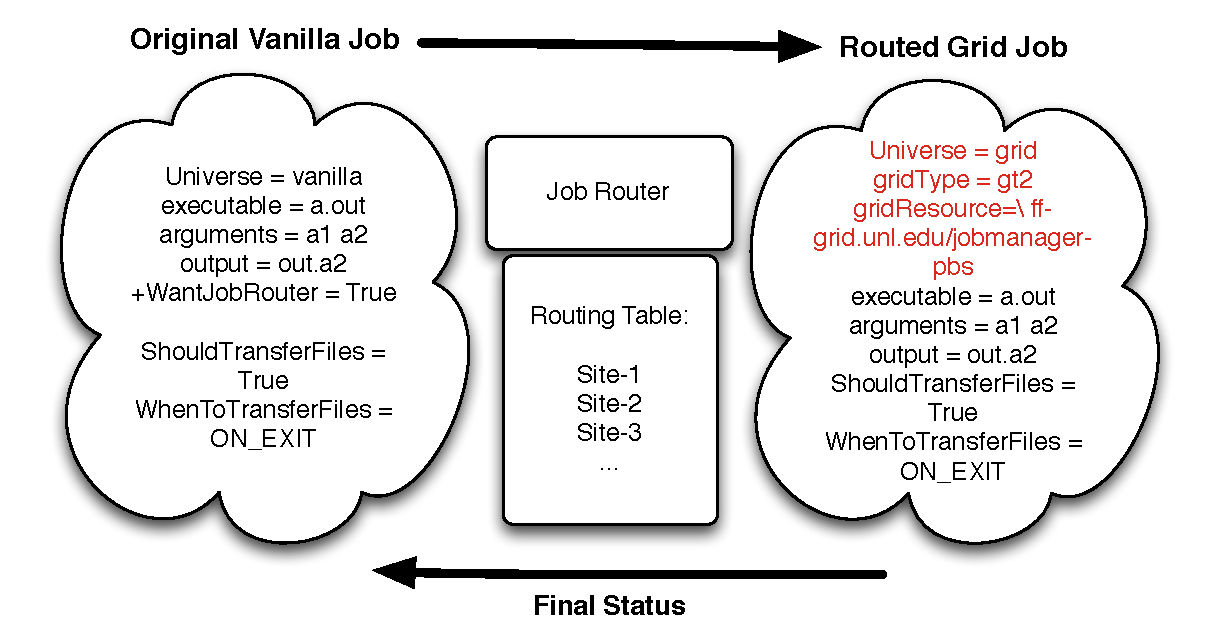
\includegraphics[scale=0.75]{images/jobRouter}
\caption{JobRouter: Transformation of Jobs}
\label{fig:JobRouter}
\end{center}
\end{figure}

A job is transformed to the grid universe by making a copy of the original job 
ClassAd, modifying some attributes of the job , this copy is called the routed 
copy and this routed copy shows up in the job queue with a new job id.

Condor job router utilizes routing table which contains the listings of sites 
the job must be submitted to and the name of the grid resource declared and 
processed during condor config file which is defined by the new ClassAds.

\begin{lstlisting}
  # Now we define each of the routes to send jobs on
JOB_ROUTER_ENTRIES = \
   [ GridResource = "gt5 ff-grid.unl.edu/jobmanager-pbs"; \
     name = "Firefly"; \
   ] \
   [ GridResource = "gt5 tusker-gw1.unl.edu/jobmanager-pbs"; \
     name = "Tusker"; \
   ] \
   [ GridResource = "gt5 pf-grid.unl.edu/jobmanager-condor"; \
     name = "Prairiefire"; \
   ]\

\end{lstlisting}


Condor Job Router seems to be a step up from the Condor Flocking in terms of 
scavenging resources and sending the extra jobs to another condor pool. Condor 
Job Router also maintains the rate of the jobs on submit hosts equal to that of remote clusters But the job 
router does not keep track of how fast each condor cluster is. Thus 
condor job router does not optimize the displacement of jobs to slower 
cluster. Since it maintains the rate of submission of jobs, we can be sure that if a job is complete 
at a faster site, its immediately replaced by the next one. The same is true for a job at slower site too
which might result in increasing the degradation if there exists some, for example if the job router kept track of slower sites, it
can send less jobs to slower sites and thereby increasing the overall throughput of the given workflow.

A preliminary examination shows that condor job router does seem to have degradation detection features, 
it does not submit to a pool that already has idle jobs but a close examination reveals that even though it
submits to a pool with non-idle jobs it isn't aware of the fact that the jobs in the queue would have 
undergone degradation due to contention on same resource and thus isn't a viable mechanism for degradation detection.
  
\subsection{Co-Scheduler Solution}
Due to the heterogeneous nature of the grid there could be problems with resource sharing on the grid. I 
came up with a solution that primarily solves the problem of degradation due to contention among 
jobs for any given resource like RAM,I/O and network. The contention among jobs sometimes give rise to 
degradation depending upon the availability of the resource that results in reduced performance of the cluster or crashes the cluster
altogether. Efficient and high throughput
distribution of jobs across multiple cluster is another challenging problem that we have solved in 
this particular Co-Scheduler Solution. 

In the first part of the solution we target the basic problem of degradation to give an example, suppose
we have a file server that can serve 100 MBps of data which is available for concurrent access and user has submitted 200 jobs
each consuming 10 MBps of data I/O. If 100 CPU slots are available, a typical state of the art Scheduler
schedules these 200 jobs without actually looking at the I/O load. This results in a degraded system, 
overtime if more jobs are Scheduled to utilize this file server. This file serve might even crash. We would need a 
degradation handling mechanism that would adaptively scale with the load and  exponentially 
backoff during high contention period thus we need an intervention in the form
of Co-Scheduler that intelligently handles degradation. 
We start the capacity algorithm by submitting jobs to the cluster and measure 
the turnaround time of each iteration if we find that the current turnaround 
time of an iteration is 25\% greater than the previous iteration we term it as a 
degradation. We now try to find the best capacity of jobs between the current 
and the previous iteration by exponentially backing-off between these two iteration. We keep finding the optimal
capacity dynamically for each iteration as the contention may change and optimal capacity keeps 
 varying. Once the optimal capacity is found then it is retained for job submission for random amount of time
 limited to maximum of ten iterations of jobs thus solving the problem of performance degradation. 
 
    
The other problem that we tackled was that of efficient distribution of work load to multiple sites of the 
grid.
Some of these sites could be error prone, some of them could be faster and some more can be slower. We need to
take an approach that improves the overall throughput of the workload, thus we keep track of average turnaround
 time for each batch of jobs submitted to the cluster. We take average of turnaround time of the batch of job that is submitted 
 across multiple cluster we group turnaround times of these batches of jobs based on the value of the 
 turnaround time to be greater than, lesser than or equal to the average turnaround time of all batch of jobs.
 This gives us a classification of sites that run faster, we exploit this information in our scheduler. 
 To implement multi-site jobs submission and load balancing feature we start submitting one job to each cluster 
 and measure the turnaround time once the job returns. Now we have the information of turnaround time 
 of a particular resource of all the clusters. Continuing to submit jobs concurrently in a similar manner
  would result in the completion of
 the workload in a non efficient way. Out of the list of all the turnaround time of different sites we take the 
 sites
 that have lower than the average turnaround time of all batches of jobs and increase the job propagation 
 factor for these jobs. This in-turn increases the number of jobs submitted to that site and helps us efficiently distribute 
 workload to faster clusters than the slower clusters ( submitting to faster site would enable us to submit 
 more
  number of jobs to the particular site. As the turnaround time is lower we would finish jobs quickly and make room for more number 
  of jobs if we submit less to slower sites that can in turn help us improve the throughput to a greater extent by enabling us to stop
  further degradation at those sites and help us submit more to faster sites .
  ) 
  Error handling mechanism is gracefully handled by 
 condor and by this approach we have an efficient system with increased throughput and with proper distribution
  of load across multiple clusters.  
        
 
 
 
 
%%A table of comparison among all three kinds of mechanisms



\section{Turnaround time based scheduling, IIT Roorkee}

\chapter{Design and Implementation of Co-Scheduler}
%(an image to showcase layer of position of co-scheduler)
The co-scheduler requires the presence of a condor installation and libcondorapi.
It is written in the C++ language and has extensively made use of pthreads for 
synchronization and multithreading. The co-schedule has two components to it,the first one is capacity detection
algorithm which is found by measuring degradation and other aspect to it is 
multi-site workload distribution across grid .The following  paragraphs detail the 
engineering aspect of the design.
The program begins by taking number of jobs, sites information and submit script 
information as its input. These number of jobs are the ones submitted across 
multiple sites. The next input file contains information on the list of sites that can be used 
for load balancing in the GridResource format of the condor ClassAds API, like \emph{tusker-gw1.unl.edu/jobmanager-pbs}.
It is assumed that all the sites listed in the sites input file are working and 
do not have any misconfiguration issues. The third and the final option to the 
scheduler is the submit description file. All the job ClassAd information and 
requirements can be written in this section and all of these will be applicable on the grid when a particular job is 
scheduled. The two main important attributes required in the submit description 
file is \emph{universe} which needs to be grid, all the time as we are submitting 
to grid sites and the other most important thing is the 
\emph{grid-proxy}. 
As we know that \texttt{condor\_wait} can be used to wait for a certain job or 
number of jobs to complete, it watches the log file and sees if the completion 
entry of the job is made in the log file that is generated by the \emph{log} 
command in the condor submit description file. There are two options we can 
specify to \texttt{condor\_wait} one is -num, number-of-jobs that waits
till the number-of-jobs are completed and the other option is to specify -wait, seconds that 
waits for seconds amount of time, if nothing is specified \texttt{condor\_wait} waits indefinitely till
the job(s) are complete.

\section{Capacity based scheduling}

This algorithm detects degradation and once we detect degradation we find the 
optimal capacity:

\begin{algorithm}
\begin{algorithmic}
\STATE $c2 \gets 1.25$ 
\COMMENT {c2: Degradation factor}
\WHILE{true}

\IF{T2 $<$ c2*T1}
  \STATE $jobSubmission(k)$ 
  %\COMMENT {Submit k jobs}
  \STATE $T1=(T1+T2)/2$
\ENDIF

\IF{T2 $>$ c2*T1}
  \STATE $degradation\_high \gets k$
  \STATE $degradation\_low \gets k/2$
  \STATE $optimalCapacity(degradation\_high,degradation\_low)$
\ENDIF

\ENDWHILE

\end{algorithmic}
\caption{Algorithm for determining optimal capacity by detecting degradation}
\label{alg:Degradation Detection}
\end{algorithm}


\begin{algorithm}
\begin{algorithmic}

\STATE $mid \gets (high+low)/2$ 
\STATE $k \gets mid$
\STATE $jobSubmission(k)$ 

\IF{T2 $<$ c2 * T1}
\STATE $T1 \gets (T1+T2)/2$
\STATE optimalCapacity(mid,high);
\ENDIF  
\IF{T2 $>$ c2 * T1}
\STATE optimalCapacity(low,mid);
\ENDIF
\RETURN mid
\end{algorithmic}
\caption{Algorithm for determining optimal capacity by detecting degradation}
\label{alg:optimalCapacity(high,low)}
\end{algorithm}


Diagram:

\section{Multi-site load distribution based scheduling}
Multi-site load distribution based scheduling uses the turnaround time at each 
site for sending future jobs, its a threaded algorithm, the following is extracted function per thread:

\begin{algorithm}
\begin{algorithmic}

\STATE $c1 \gets 2$ 
\COMMENT {c1: Job propagation factor}

\STATE $high \gets 0$
\STATE $low \gets 0$
\STATE $average \gets 0$

\COMMENT {arrayMultipleSitesTime is populated with turnaround times of all sites}
\STATE $arrayMultipleSitesTime.sort()$
\STATE $low = arrayMultipleSitesTime.front()$
\STATE $high = arrayMultipleSitesTime.back()$
\STATE average = SUM(arrayMultipleSitesTime) / Sizeof(arrayMultipleSitesTime)

\IF{turnaroundTime\_Thread $==$ low}
\STATE $c1 \gets c1 * 4$
\ENDIF

\IF{turnaroundTime\_Thread $==$ high}
\STATE $c1 \gets c1/2 ? (c1/2:1)$
\ENDIF

\IF{turnaroundTime\_Thread $<$ average}
\STATE $c1 \gets c1 * 2$
\ENDIF

\end{algorithmic}
\caption{Algorithm for distribution of workflow load across multiple sites on the grid}
\label{alg:updateJobPropagationConstant()}
\end{algorithm}


\begin{figure}[htbp!]
\begin{center}
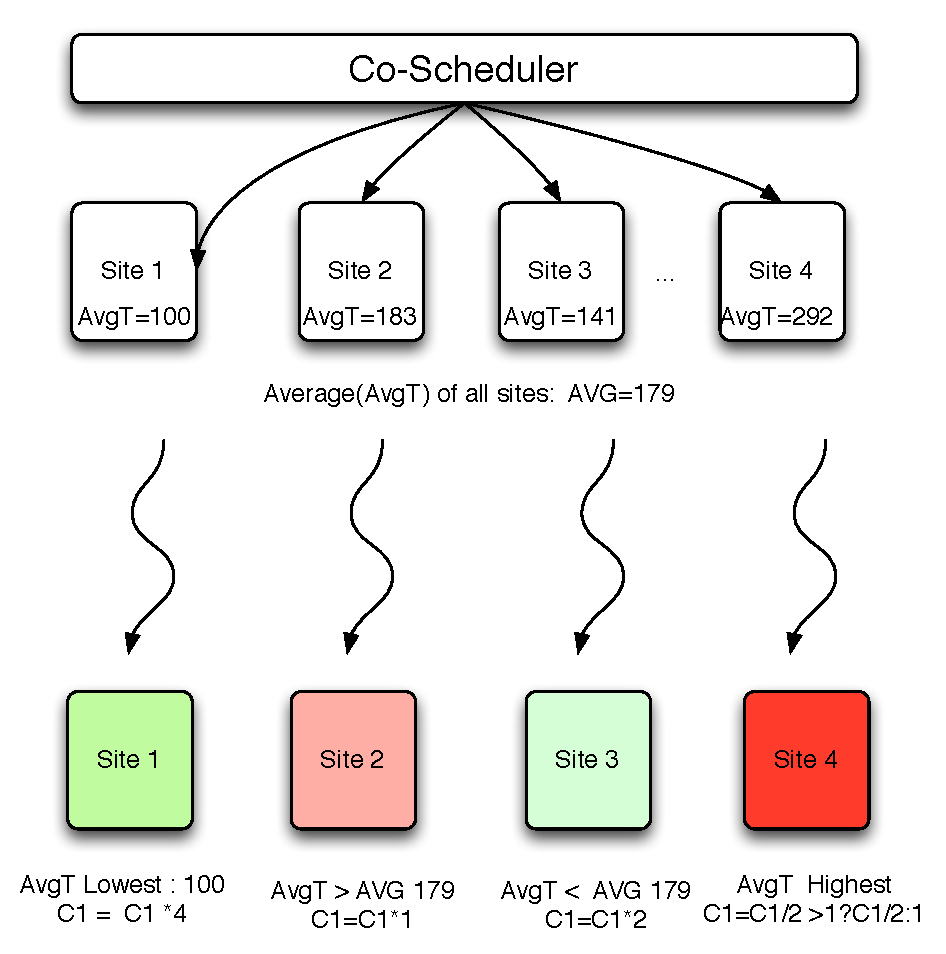
\includegraphics[scale=0.75]{images/multipleSites}
\caption{Multi-site scheduling algorithm overview, classification of sites into slower and faster}
\label{fig:multiSite1}
\end{center}
\end{figure}
\FloatBarrier
Diagram:
\section{Programming APIs}
\subsection{Condor Log Reader and User API}

Condor provides Job Log Reader API that polls logs for job events by giving us 
API access to the events and outcomes. The following is the constructor for 
initializing a ReadUserLog object.

Constructor:
ReadUserLog reader(fp,false,false);
\begin{verbatim}
ULogEventOutcome (defined in condor_event.h):

Status events for job detection:

ULOG_OK: Event is valid
ULOG_NO_EVENT: No event occurred (like EOF)
ULOG_RD_ERROR: Error reading log file
ULOG_MISSED_EVENT: Missed event
ULOG_UNK_ERROR: Unknown Error
\end{verbatim}

All the entries in the log file end with \texttt{...}. All the job 
log entries as named as events and these events could range form being  \texttt{ULOG\_OK} where 
the event has taken place and is valid to \texttt{ULOG\_UNK\_ERROR} where an error has 
taken place.

The following pauedo-code is an extract from the logReader function that first 
detects all the valid events and then based on the data-structure of the event 
object detects if the event kind is \texttt{ULOG\_EXECUTE} meaning the job has begun 
executing via eventNumber data member. Finally we detect the \texttt{ULOG\_JOB\_TERMINATED} 
event where job has successfully terminated. We also cast more general event 
object into JobTerminatedEvent to access data members of the JobTerminatedEvent.


Job Submission Psuedo-Code:

\begin{lstlisting}
void logReader(string hostFile, args *data, int nSites)	{		
		FILE *fp;
		ReadUserLog reader(fp,false,false);
		ULogEvent *event = NULL;		
             while(reader.readEvent(event)==ULOG_OK)	{                    
            if((*event).eventNumber==ULOG_EXECUTE )	{                                
            //Cast into Execute Event
                ExecuteEvent *exec 
                = static_cast<ExecuteEvent*>(event);                                       
                //condor_wait -num K, where K is the 
                //amount of jobs completed till the wait.
                    char tmp[100];
                    sprintf(tmp,"condor_wait -num 
                    \%d \%s",count,hostFile.c_str());
            }            
            if((*event).eventNumber==ULOG_JOB_TERMINATED)	{                
            //Cast into Job Terminated Event
                JobTerminatedEvent *term 
                = static_cast<JobTerminatedEvent*>(event);                
                
                if(term->normal)	{                    
                    //on Normal termination, works only for local jobs, 
                    //find the CPU time of local jobs
                }               
            }
        }
}

\end{lstlisting}
\subsection{Synchronization Co-Scheduler Code}

There are critical sections in the code where synchronization becomes absolutely 
necessary. One such variable is number of jobs. Number of jobs executed across 
the sites should remain fixed and the value must match the value that has been 
given as input. In a threaded system where each thread is executing on a 
different cluster it becomes necessary to define \texttt{N}, number of jobs executed or executing as a 
critical section. Here we define a pthread mutex and lock it for all write accesses to the \texttt{N}
and serialize the access to \texttt{N} and make conditional checks during job submission, not to allow
job submissions when \texttt{N} is greater than input value. By 
serializing the access across multiple threads the total jobs executed remains 
equal to the input number of jobs. The following chunk of code block 
demonstrates the use of mutexes for serialization of  \texttt{N} among the threads.

Another section of code where synchronization becomes important is while 
distributing the jobs to multiple sites. We're measuring which cluster is 
faster, in doing so we need information of turnaround time from all the sites 
before proceeding that means all the threads need to be executing a line of code 
before proceeding with the further program. Thus the absolute need for 
synchronization. To handle this problem we make use of conditional variable of 
pthread. The following chunk of code demonstrates the use of conditional wait 
and conditional signal variable that clears the block on all the threads waiting 
based on the given condition.

\chapter{Evaluation}

\chapter{Conclusion}


%% backmatter is needed at the end of the main body of your thesis to
%% set up page numbering correctly for the remainder of the thesis
\backmatter

%% Start the correct formatting for the appendices
\appendix

%% Appendices go here (if you have them)

%% Bibliography goes here (You better have one)
%% BibTeX is your friend
%% Index go here (if you have one)
%% Bibliography goes here (You better have one)
%% BibTeX is your friend
\bibliographystyle{plain}
\bibliography{KartikThesis}
%% Pull in all the entries in the bibtex file. Is is a useful trick to
%% check all your references.
\nocite{*}

%% Index go here (if you have one)

\end{document}